\documentclass[10pt]{article}
\usepackage{icmlko}

\icmlmeta{IP 파운데이션 월드모델}{232}{한 행이 도메인을 죽였다}{노트 231이 기준선이 죽은 것을 찾고 가드를 세웠다. 왜 죽었는지는 안 봤다. 짐작 셋이 틀리고 넷째에서 계측했더니 하네스 한 줄이었다}

\begin{document}

\twocolumn[
\icmlheader

\begin{abstract}
노트 231이 ``F1 이 아홉 도메인 중 여덟에서 죽었다''를 찾고 덮음 보고와
가드를 세웠지만 \textbf{왜 죽었는지는 안 봤다.} 봤다. \textbf{짐작 셋이
차례로 틀렸다.} ① 완전사례 필터 --- \texttt{\_keep\_rows} 를 그대로
적용하니 \emph{모든} 축 판에서 8/10 도메인이 20행 이상 남는다. ② F1 내부
--- 도메인별 분해와 쌍별 정렬이 두 축 판 모두에서 7$\sim$9개 출처에
성공한다. ③ 출처 부족 --- 9/10 도메인이 출처가 된다(못 되는 것은 팝업
하나, 학습 16행). \textbf{넷째로 계측해서 찾았다: \texttt{scipy.rankdata}
의 기본 정책이 NaN 전파다.} \texttt{rank.predictions} 가 예측 벡터에
\texttt{rankdata} 를 그대로 걸어서, \textbf{못 매기는 행을 정직하게 NaN
으로 돌려주는 정식화가 도메인 \emph{전체}를 잃는다.} 크기가 이렇다 ---
\textbf{웹툰은 711건 중 7건을 못 매겨서 711건을 다 잃는다.} 애니 21/606 ·
도서 2/163 · 팝업 5/59 도 마찬가지고, 살아남은 것은 버린 행이 정확히
0 인 펀딩 하나였다. 노트 231이 본 ``판 $+$0.1472'' 가 바로 그
펀딩 80건이다. 고쳤다 --- \texttt{\_rank\_nan} 은 유한한 것만 순위 매기고
나머지는 NaN 으로 둔다. \textbf{부분 결측은 부분으로 남아야
\texttt{coverage} 가 무엇이 빠졌는지 적을 수 있다.} 효과가 정확히
갈린다: \textbf{F1 이 1/9 도메인(표본 80)에서 8/9(2,230)로 부활하고 판이
$+$0.1472 $\to$ $+$0.2447} 인데, \textbf{살아 있던 것들은 소수 넷째
자리까지 안 움직인다}(F21 $+$0.4321 · F18 $+$0.4523). \textbf{노트 187의
제일 값싼 검사를 반대로 쓴 것이다} --- 거기서는 ``안 움직이면 안 닿은
것''이었고 여기서는 \textbf{``안 움직여야 맞는 것''}이다.
\end{abstract}
]

\begin{figure*}[t]
\centering
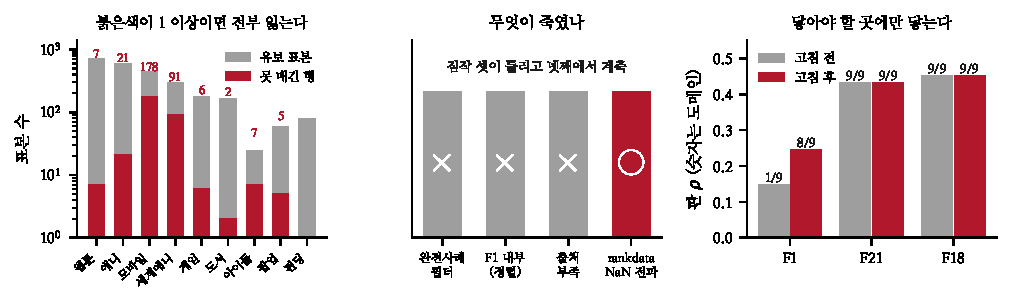
\includegraphics[width=\textwidth]{figs/onerow.pdf}
\caption{왼쪽 --- 못 매긴 행이 하나라도 있으면 전부 잃는다. 가운데 ---
짐작 셋이 틀렸다. 오른쪽 --- 고침이 닿아야 할 곳에만 닿는다.}
\end{figure*}

\section{짐작 셋이 틀렸다}

\begin{table}[t]
\centering\tsize
\caption{차례로 확인한 것.}
\begin{tabular}{lll}
\toprule
짐작 & 잰 것 & \\
\midrule
완전사례 필터 & 8/10 도메인이 20행 이상 & × \\
F1 내부(정렬) & 출처 7$\sim$9개 정렬 성공 & × \\
출처 부족 & 9/10 도메인이 출처가 됨 & × \\
\textbf{rankdata NaN} & \textbf{한 행이 벡터 전체를} & \textbf{○} \\
\bottomrule
\end{tabular}
\end{table}

\claimx{\textbf{짐작 셋이 차례로 틀렸다.} 축이 늘수록 F1 이 죽는 것을 보고
``완전사례 필터가 조이는구나''로 읽었는데, 그 필터는 모든 축 판에서 8/10
도메인을 살려 둔다.}{\textbf{노트 133의 규칙이 세 번 걸렸다} --- 그리고
이번에는 판정치가 아니라 \emph{기전}에 대한 짐작이었다. 노트 218이
``결론 옆에 적은 까닭이 결론보다 잘 틀린다''를 여덟 번째로 셌고 노트 225가
아홉 번째였는데, \textbf{한 노트 안에서 세 번은 처음이다.}}

\section{한 행이 도메인 전체를 죽인다}

\begin{table}[t]
\centering\tsize
\caption{trendcalwiki 에서 F1 이 못 매기는 행.}
\begin{tabular}{lrrl}
\toprule
& 유보 & 못 매김 & 결과 \\
\midrule
\textbf{웹툰} & 711 & \textbf{7} & \textbf{711건 전부 잃음} \\
애니 & 606 & 21 & 전부 잃음 \\
모바일 & 441 & 178 & 전부 잃음 \\
세계애니 & 300 & 91 & 전부 잃음 \\
게임 & 180 & 6 & 전부 잃음 \\
도서 & 163 & \textbf{2} & 전부 잃음 \\
팝업 & 59 & 5 & 전부 잃음 \\
\textbf{펀딩} & 80 & \textbf{0} & \textbf{살아남음} \\
\bottomrule
\end{tabular}
\end{table}

\claimx{\texttt{scipy.rankdata} 의 기본 \texttt{nan\_policy} 가
\emph{전파}다. \texttt{rank.predictions} 가 예측 벡터에 그대로 걸어서
\textbf{한 행이 NaN 이면 벡터 전체가 NaN 이 된다.}}{\textbf{웹툰은 711건
중 7건 때문에 711건을 다 잃는다}(0.98\%). 도서는 2건 때문에 163건을
잃는다(1.2\%). \textbf{살아남은 것은 버린 행이 정확히 0 인 펀딩
하나이고, 노트 231이 본 ``판 $+$0.1472'' 가 그 80건이다.}}

\claimx{\textbf{F1 은 잘못한 것이 없다.} 못 매기는 행을 NaN 으로 돌려주는
것은 정직한 설계다 --- 완전사례 분해라 일부 행은 원래 점수가 없다.}
{\textbf{하네스가 그 정직함을 벌했다.} 부분 결측을 허용하지 않는 순위
함수가 ``부분''을 ``전무''로 바꿨다.}

\section{고침}

\begin{table}[t]
\centering\tsize
\caption{\texttt{\_rank\_nan} --- 유한한 것만 순위.}
\begin{tabular}{lrrrr}
\toprule
& \multicolumn{2}{c}{고침 전} & \multicolumn{2}{c}{고침 후} \\
& 판 & 도메인 & 판 & 도메인 \\
\midrule
\textbf{F1} & $+$.1472 & \textbf{1/9} & \textbf{$+$.2447} & \textbf{8/9} \\
F21 & $+$.4321 & 9/9 & $+$.4321 & 9/9 \\
F18 & $+$.4523 & 9/9 & $+$.4523 & 9/9 \\
\bottomrule
\end{tabular}
\end{table}

\claimx{\textbf{F1 이 1/9 도메인(표본 80)에서 8/9(2,230)로 부활하고
판이 $+$0.1472 $\to$ $+$0.2447 이다.} 그리고 \textbf{살아 있던 것들은
소수 넷째 자리까지 안 움직인다.}}{\textbf{노트 187의 제일 값싼 검사를
반대로 쓴 것이다} --- 거기서는 ``판이 안 움직이면 모형에 안 닿은 것''이
경고였고, \textbf{여기서는 ``안 움직여야 맞는 것''이 확인이다.} 고침이
닿아야 할 곳에만 닿았다.}

\claimx{\textbf{F1 의 진짜 기준선은 $+$0.24$\sim$0.26 이다}(base
$+$0.2591 · trendcalwiki $+$0.2447). \textbf{여전히 포트폴리오 꼴찌이고,
그것이 노트 125의 결론과 맞는다} --- 옛 파이프라인이 도전자들에게
진다.}{\textbf{다만 $+$0.1472 는 그 결론의 근거가 아니었다} --- 그 수는
펀딩 하나였다. \textbf{결론은 맞았고 근거는 우연이었다.}}

\begin{table}[t]
\centering\tsize
\caption{남은 것.}
\begin{tabular}{ll}
\toprule
\textbf{옛 수치} & F1 을 인용한 노트가 둘(125 · 126) \\
\textbf{F17} & IndexError --- 아직 안 봤다 \\
같은 병 & 부분 NaN 을 내는 다른 정식화가 있나 \\
\bottomrule
\end{tabular}
\end{table}

첫 줄은 이미 값이 작아졌다. F1 을 실질적으로 인용한 노트는 125와 126
둘뿐이고, \textbf{노트 125는 덮음을 적었다} --- 표에 도메인 수 8 이 있고
``F1 은 아이돌을 채점하지 못한다''고 본문에 썼다. \textbf{그때는 8/9 로
살아 있었고 관행도 있었다.} 그러니 이 사고는 ``덮음을 안 적어서''가 아니라
\textbf{``적던 것을 그만둬서''}다 --- 노트 125 이후 축이 셋 늘고 정식화가
열여섯 늘면서 표가 간소해졌고, 그 간소함이 기준선이 죽는 것을 백 노트
동안 가렸다. \textbf{노트 231이 붙인 덮음 보고는 그 관행을 되살리는 것이지
새로 만드는 것이 아니다.}

\end{document}
